\documentclass[conference]{IEEEtran}
\IEEEoverridecommandlockouts
\usepackage{cite}
\usepackage{amsmath,amssymb,amsfonts}
\usepackage{algorithmic}
\usepackage{graphicx}
\usepackage{textcomp}
\usepackage[utf8]{inputenc}
\usepackage{xcolor}
\usepackage{float}
\usepackage{hyperref}
\usepackage{listings}
\usepackage{subcaption}

\def\BibTeX{{\rm B\kern-.05em{\sc i\kern-.025em b}\kern-.08em
    T\kern-.1667em\lower.7ex\hbox{E}\kern-.125emX}}

\begin{document}

\title{Optimizing Emergency Fire Response Using Traffic Data in Istanbul}

\author{\IEEEauthorblockN{Furkan Karagöz}
\IEEEauthorblockA{\textit{040210008} \\
\textit{Electronics and Communication Engineering}\\
\textit{Istanbul Technical University}\\
karagozf21@itu.edu.tr}
\and
\IEEEauthorblockN{Alim Ege Uzun}
\IEEEauthorblockA{\textit{040230755} \\
\textit{Electronics and Communication Engineering}\\
\textit{Istanbul Technical University}\\
uzuna21@itu.edu.tr}
}

\maketitle

\vspace{1em}
\section*{\textbf{Author Contributions}}

\textbf{Furkan Karagöz:} Designed and implemented the Genetic Algorithm (GA) model, including the fitness function, constraint handling mechanisms, and repair operations. Contributed to comparative analysis between static and dynamic assignment models, and prepared the presentation slides.

\textbf{Alim Ege Uzun:} Processed the fire station and traffic data, implemented the Particle Swarm Optimization (PSO) algorithm, and generated the travel time matrices. Structured the LaTeX report and handled the dynamic demand zone clustering using K-Means and critical point selection.

\vspace{1.5em}





\begin{abstract}
In large metropolitan cities like Istanbul, providing rapid fire emergency response is a challenging operational problem mainly due to highly dynamic traffic conditions. This project proposes a data-driven optimization framework that assigns fire stations to urban demand zones by explicitly considering both real-time traffic and station capacity constraints. Unlike traditional static models based solely on geographic proximity, our approach leverages real travel time data and uses metaheuristic algorithms—Particle Swarm Optimization (PSO) and Genetic Algorithm (GA)—to minimize the total and worst-case response times across the city. The assignment problem is solved for different hours of the day to reflect traffic variability. The results show that dynamic optimization models significantly reduce the total cost and are much more practical compared to basic static assignments. Our findings demonstrate the value of integrating real-world constraints and live data into emergency response planning, providing practical insights for smarter and safer urban fire management.
\end{abstract}

\section*{\textbf{Problem Statement}}
Fast and effective emergency response is a critical requirement in large urban areas where traffic congestion and complex urban layouts can significantly delay response times, especially in fire incidents. In Istanbul, one of the most densely populated and traffic-intensive megacities in the world, minimizing fire response time is not only a matter of service quality, but also a vital factor that can save lives and property. The main problem addressed in this project is to optimally assign fire stations to urban demand zones in a way that minimizes response times, taking into account real-time traffic conditions and the limited capacities of each station. Unlike traditional static assignment models that usually allocate demand only according to geographical distance or static road networks, this study incorporates dynamic traffic data and practical operational constraints. The challenge is further compounded by the spatial distribution of fire stations, the change in traffic speeds throughout the day, and the limited number of vehicles and personnel available at each station. The problem then becomes a constrained combinatorial optimization problem: How can we assign each demand zone to a fire station so that response times are minimized, station overloads are prevented, and the solution remains applicable under real city conditions. This research aims to develop and validate a data-driven, optimization-based approach to fire station assignments in Istanbul, providing a more realistic and effective alternative to existing static planning methods.
\section*{\textbf{Hypothesis}}

We hypothesize that incorporating real-time traffic conditions and fire station capacity constraints into the assignment process will significantly improve emergency response effectiveness in urban environments. Specifically, we assume that metaheuristic optimization algorithms such as Particle Swarm Optimization (PSO) and Genetic Algorithm (GA) can produce more efficient and realistic fire station-to-demand zone assignments compared to traditional static, distance-based models. Moreover, we expect that these dynamic models will better adapt to temporal variations in traffic and operational limitations, leading to reductions in both average and worst-case response times.

\section*{\textbf{Literature Survey}}

The optimization of emergency response logistics has long been an area of active research, especially in large urban environments. Traditional methods often rely on static models based on Euclidean distance or fixed response regions, which fail to account for real-world factors such as traffic congestion, road conditions, and station capacities. Recent studies have begun to address these limitations by integrating data-driven and heuristic approaches.

Metaheuristic algorithms, including Genetic Algorithm (GA) and Particle Swarm Optimization (PSO), have been applied to various public service optimization problems. Studies like Li et al. (2019) and Zhang et al. (2020) have demonstrated that these techniques outperform greedy or purely deterministic methods when handling dynamic inputs and constraints. In the context of emergency services, works by Gendreau et al. and Huang et al. highlight the importance of considering real-time travel times and resource constraints.

However, most of these studies either oversimplify the problem or lack scalability for high-demand zones. Our project builds upon these foundations by incorporating both real-time traffic data and fire station vehicle capacities, addressing a crucial gap in emergency response optimization literature.
\section*{\textbf{Methods}}
\subsection{\textit{ Particle Swarm Optimization }}
This project seeks to improve upon these limitations by developing a traffic-aware, dynamic assignment model. The city is divided into a finite number of demand zones $Z = \{z_1, z_2, ..., z_n\}$, each of which requires emergency coverage. A fixed set of fire stations $S = \{s_1, s_2, ..., s_m\}$ is available to serve these zones. Each pair $(s_i, z_j)$ has an associated estimated travel time $T_{ij}$, derived from historical or real-time traffic data.

We define a binary decision variable $x_{ij}$ as follows:

\[
x_{ij} =
\begin{cases}
1 & \text{if demand zone } z_j \text{ is assigned to fire station } s_i \\
0 & \text{otherwise}
\end{cases}
\]

Objective function:
\begin{itemize}
  \item Minimize total expected travel time:
  \[
  \min \sum_{i=1}^{m} \sum_{j=1}^{n} T_{ij} \cdot x_{ij}
  \]
\end{itemize}

Particle Swarm Optimization is a population-based metaheuristic inspired by the social behavior of birds and fish. Each particle in the swarm represents a candidate solution (i.e., a zone-to-station assignment vector). The particles "fly" through the search space and adjust their positions based on their own experience and the experience of their neighbors.

\begin{itemize}
  \item \textbf{Encoding:} Each particle encodes a vector of length $n$, where each index represents a demand zone and the value indicates the assigned station.
  \item \textbf{Fitness Function:} Combines average response time and worst-case response time, using a weighted objective as described in Section II.A. Constraint violations (e.g., capacity) are penalized using additive penalty terms.
  \item \textbf{Velocity Update Rule:}
  \[
  v_i^{(t+1)} = w \cdot v_i^{(t)} + c_1 \cdot r_1 \cdot (p_i - x_i^{(t)}) + c_2 \cdot r_2 \cdot (g - x_i^{(t)})
  \]
  where $w$ is inertia weight, $p_i$ is the particle’s best known position, and $g$ is the global best.
\end{itemize}

We observed the optimization of station-demand zone assignments obtained from traffic data at 2 and 10 o'clock using particle swarm optimization algorithm and compared it with static assignment based on Euclidean distance. In the static assignment approach, the station-demand zone distance is calculated using Euclidean distance, then divided by a predetermined average speed to compute static travel time. 

The dynamic model incorporates both capacity constraints and traffic effects realistically, producing more balanced and feasible assignments. While the static model theoretically provides the "shortest" path solution, it often fails under real-world constraints - when capacity limits or traffic effects are considered, these assignments frequently break down, leading to total additional costs reaching up to 30\%. 
In contrast, the dynamic model's solutions better reflect real-world conditions, maintaining lower additional costs in the range of 18-19\%.

This demonstrates the static model's practical insufficiency and over-optimism, while confirming that the dynamic approach yields more realistic and robust solutions. The results clearly show that accounting for dynamic factors is essential for effective station-demand zone assignment in actual operating conditions.


\begin{figure}[htbp]
    \centering
    \begin{subfigure}[b]{0.48\textwidth}
        \centering
        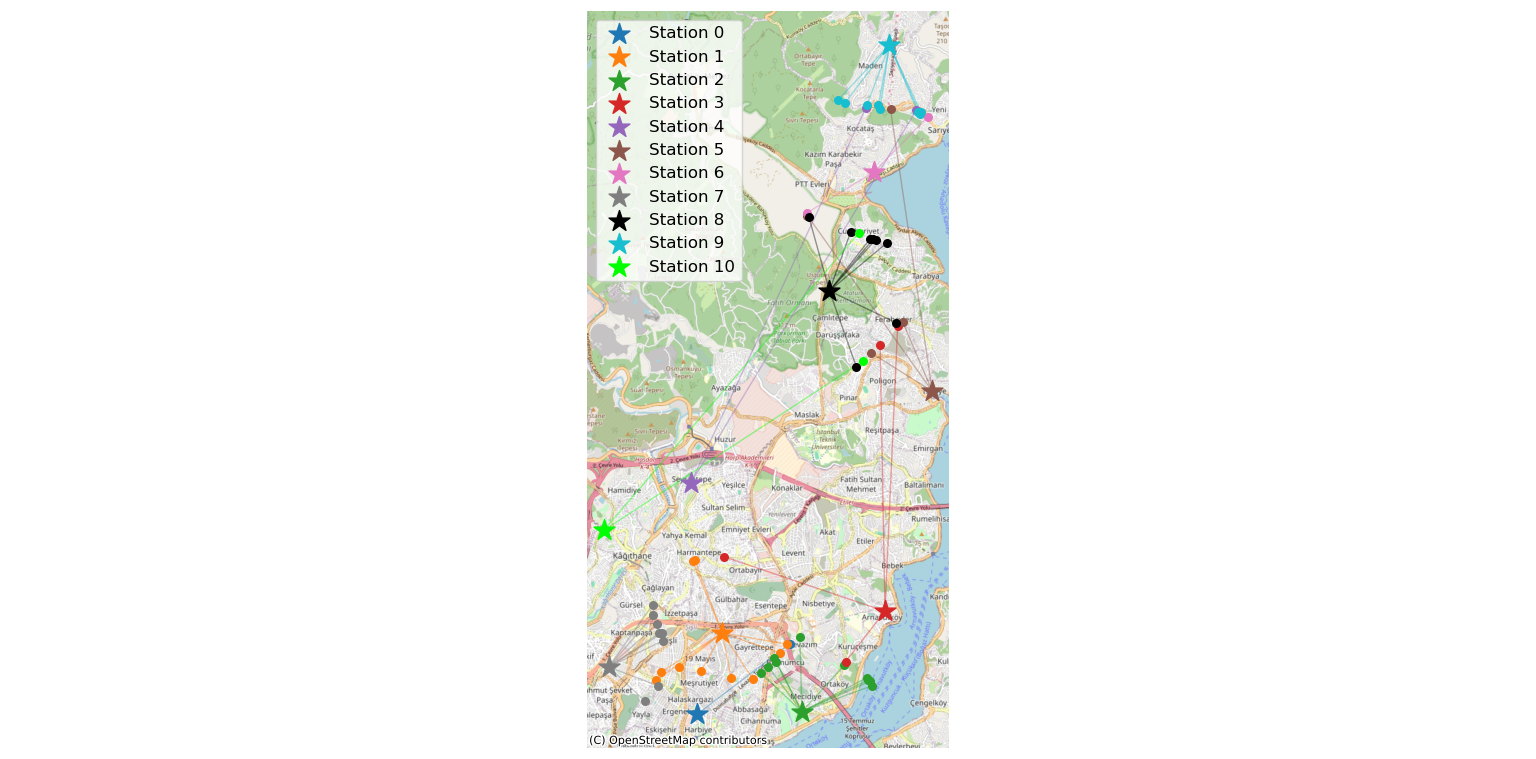
\includegraphics[width=\linewidth]{pso_map (1).png}
        \caption{PSO with traffic data (2 AM)}
        \label{fig:pso_dynamic}
    \end{subfigure}
    \hfill
    \begin{subfigure}[b]{0.48\textwidth}
        \centering
        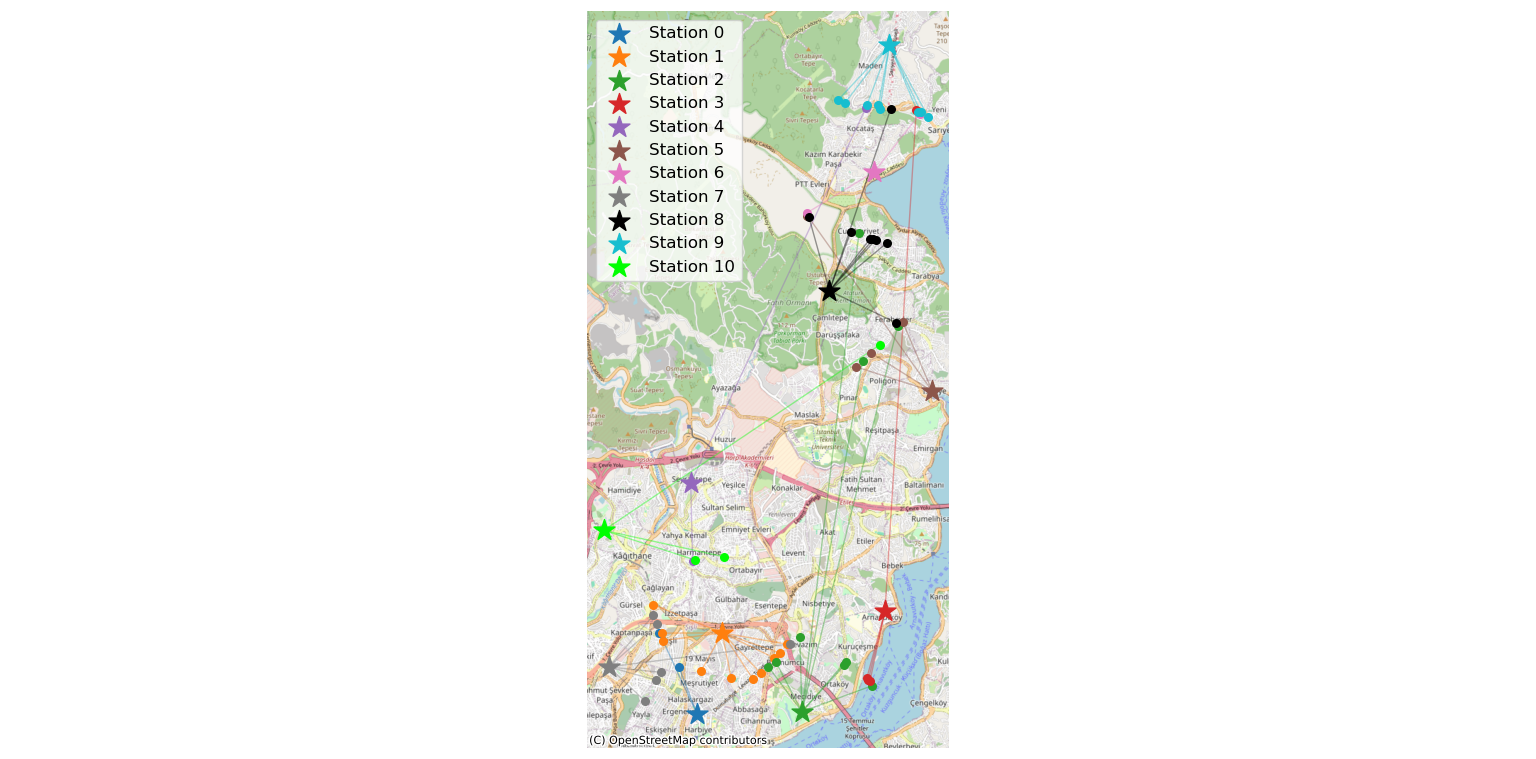
\includegraphics[width=\linewidth]{pso_static_map (1).png}
        \caption{PSO with static assignment}
        \label{fig:pso_static}
    \end{subfigure}
    
    \vspace{1em}
    
    \begin{subfigure}[b]{0.48\textwidth}
        \centering
        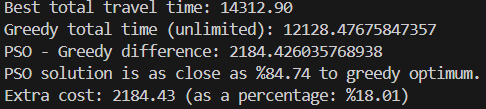
\includegraphics[width=\linewidth]{pso_result.png}
        \caption{Results with traffic data}
        \label{fig:pso_dynamic_result}
    \end{subfigure}
    \hfill
    \begin{subfigure}[b]{0.48\textwidth}
        \centering
        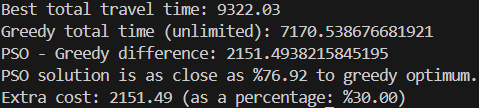
\includegraphics[width=\linewidth]{pso_static_result.png}
        \caption{Static assignment results}
        \label{fig:pso_static_result}
    \end{subfigure}
    
    \caption{PSO optimization results: (a-b) Assignment maps, (c-d) Performance metrics}
    \label{fig:pso_results}
\end{figure}

\subsection{\textit{Genetic Algorithm (GA)}}
A Genetic Algorithm (GA) was implemented to optimize fire station assignments, with its detailed logic and experiments documented in the \texttt{ga\_deneme\_1.ipynb} notebook. The GA, inspired by natural selection, evolves a population of candidate solutions (chromosomes) over generations to identify optimal or near-optimal assignments. This study primarily focuses on GA performance using travel time data for 2 AM to clearly illustrate the differences between assignments based on static assumptions versus those incorporating dynamic, low-traffic travel times. The analyses were conducted for two distinct sets of 80 demand points: zones selected via K-means clustering (\texttt{kmeans80}) and critically selected demand zones (\texttt{critical\_points}).

\begin{itemize}
    \item \textbf{Chromosome Representation and Encoding:} Each chromosome represents a complete assignment of $N_d=80$ demand zones to one of $N_s=11$ fire stations. It is encoded as a one-dimensional array where the $j$-th element indicates the fire station index assigned to demand zone $z_j$.

    \item \textbf{Initialization of Population (\texttt{init\_population}):} The initial population of \texttt{pop\_size = 100} chromosomes is generated by including one greedily assigned solution and filling the rest with random assignments. All initial solutions are processed by a \texttt{repair\_assignment} function to meet capacity constraints.

    \item \textbf{Fitness Function (\texttt{fitness\_function}):} The fitness of an assignment is evaluated using a weighted sum of the total travel time and the worst-case travel time, plus penalties for constraint violations:
    \[ \text{Fitness} = \alpha \times \left(\sum_{j=1}^{N_d} T_{s_j, j}\right) + (1 - \alpha) \times \left(\max_{j} T_{s_j, j}\right) + \text{Penalty} \]
    where $T_{s_j, j}$ is the travel time for demand zone $j$ assigned to station $s_j$, and $\alpha = 0.8$. Penalties are applied for exceeding station capacities and for assignments with infinite travel times. For the \texttt{critical\_points} dataset, station capacities were set to \texttt{[10, 10, 10, 4, 2, 4, 2, 8, 8, 8, 4]}, while for the \texttt{kmeans80} dataset, they were \texttt{[8, 10, 10, 8, 6, 6, 6, 8, 6, 6, 8]}. The penalty for capacity violation is $10000 \times \sum (\text{overload\_amount})$, and for infinite travel time, it is $100000$.

    \item \textbf{Repair Mechanism (\texttt{repair\_assignment}):} A repair function ensures solution feasibility by reassigning demand zones from overloaded stations to those with available capacity, prioritizing minimal travel time. This is applied after initialization and genetic operations.

    \item \textbf{Selection (\texttt{tournament\_selection}):} Parents are chosen using tournament selection with a tournament size of $k=3$.

    \item \textbf{Crossover (\texttt{crossover}):} Single-point crossover is applied with a probability of \texttt{crossover\_rate = 0.9}. Offspring are subsequently repaired.

    \item \textbf{Mutation (\texttt{mutate}):} Each gene is mutated with a probability of \texttt{mutation\_rate = 0.15}, reassigning the demand zone to a random station. Mutated individuals are then repaired.

    \item \textbf{Elitism:} The top \texttt{elite\_count = 2} individuals from each generation are carried to the next.

    \item \textbf{Parameters and Termination:} The GA runs for \texttt{max\_gen = 100} generations. Key parameters for both K-Means and Critical Points experiments at 2 AM included: population size = 100, crossover rate = 0.9, mutation rate = 0.15, and elite count = 2.
\end{itemize}
The GA was applied using both static $T_{ij}$ matrices (based on Euclidean distances and average speeds) and dynamic $T_{ij}$ matrices calculated for 2 AM traffic conditions. The resulting optimal assignment maps and quantitative performance metrics for these scenarios are presented in Table \ref{tab:ga_results} and Figures \ref{fig:ga_assignments_kmeans}--\ref{fig:ga_assignments_critical} to illustrate the impact of different demand point selection strategies and the effect of incorporating dynamic travel time data.

% Quantitative Results Table
\begin{table}[htbp]
\centering
\caption{GA Performance Metrics for Different Datasets and Travel Time Models}
\label{tab:ga_results}
\begin{tabular}{lcccrr}
\toprule
\textbf{Dataset} & \textbf{Model} & \textbf{GA Time (s)} & \textbf{Greedy (s)} & \textbf{Extra Cost} & \textbf{Met?} \\
\midrule
Critical & Static & 9,322.83 & 7,270.52 & 2,052.31 (28.2\%) & Yes \\
Critical & 2 AM & 14,312.90 & 12,128.48 & 2,184.42 (18.0\%) & Yes \\
K-Means & Static & 31,335.51 & 15,650.89 & 15,684.62 (100.2\%) & Yes \\
K-Means & 2 AM & 43,556.57 & 24,150.52 & 19,406.05 (80.4\%) & Yes \\
\bottomrule
\end{tabular}
\end{table}

Table \ref{tab:ga_results} summarizes the quantitative performance of the GA across different scenarios. Key observations include:
\begin{itemize}
    \item The K-Means dataset consistently resulted in higher total travel times (31,335-43,556 seconds) compared to the Critical Points dataset (9,322-14,312 seconds), regardless of the travel time model used
    \item Both datasets showed increased travel times when using the dynamic 2 AM model compared to the static model, with the K-Means dataset showing a more pronounced increase (39\% increase vs 53\% increase for Critical Points)
    \item The GA successfully satisfied all capacity constraints in all scenarios, demonstrating the effectiveness of the repair mechanism
    \item The extra cost (difference between GA solution and unconstrained greedy optimum) was substantial in all cases, highlighting the impact of capacity constraints
\end{itemize}

Figure \ref{fig:ga_assignments_kmeans} compares the optimal assignments for the 80 demand zones selected via K-means clustering. Subfigure \ref{fig:ga_kmeans_static_map_only} shows the assignments when using a static $T_{ij}$ matrix (Total Time = 31,335.51 s), where allocations are largely influenced by geographical proximity. In contrast, Subfigure \ref{fig:ga_kmeans_map_saat2_only} displays the assignments derived from the 2 AM traffic-aware $T_{ij}$ matrix (Total Time = 43,556.57 s). Noticeable shifts in zone-to-station allocations can be observed, indicating that even under low-traffic conditions, dynamic travel times lead to different optimal coverage strategies compared to purely static assumptions.

% --- GA K-Means: Static vs Saat 2 AM Maps ---
\begin{figure}[htbp]
    \centering
    \begin{subfigure}[b]{0.49\textwidth}
        \centering
        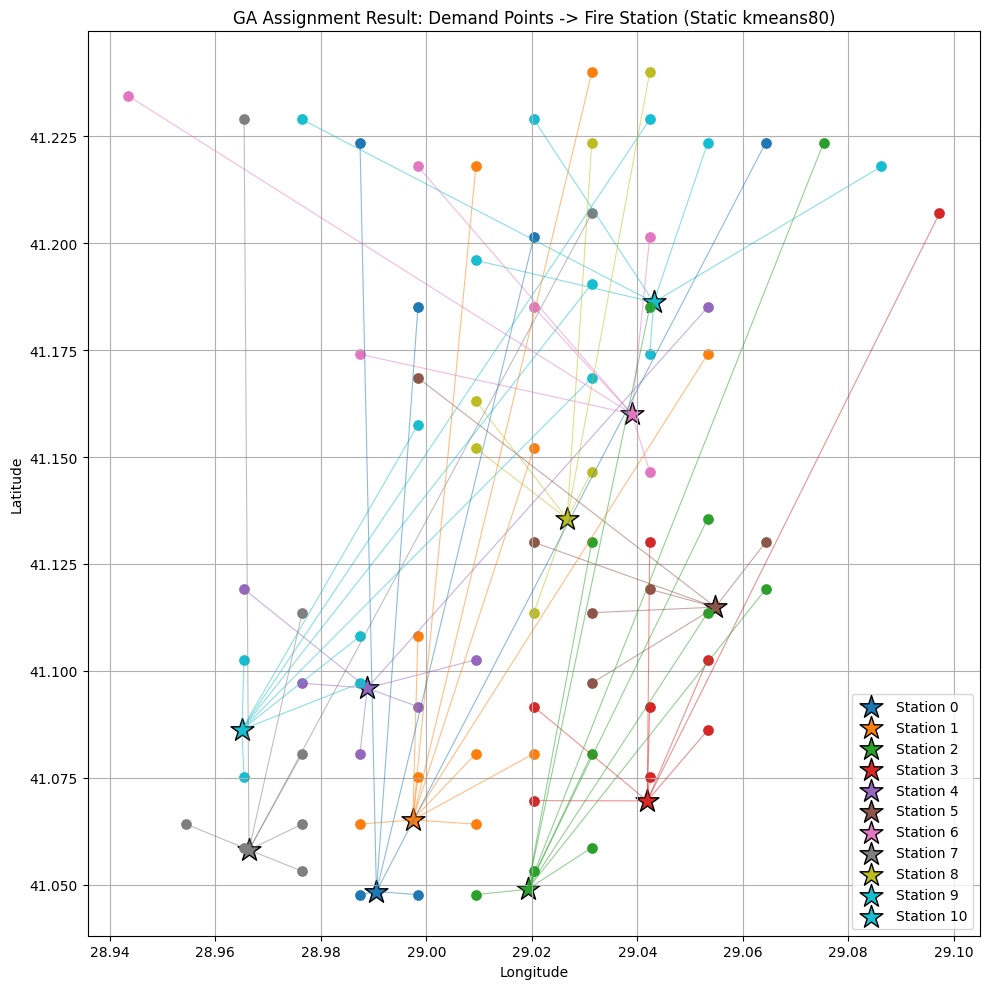
\includegraphics[width=\linewidth]{ga_kmeans_static_map.png}
        \caption{Static Model Assignment (K-Means Points)}
        \label{fig:ga_kmeans_static_map_only}
    \end{subfigure}
    \hfill
    \begin{subfigure}[b]{0.49\textwidth}
        \centering
        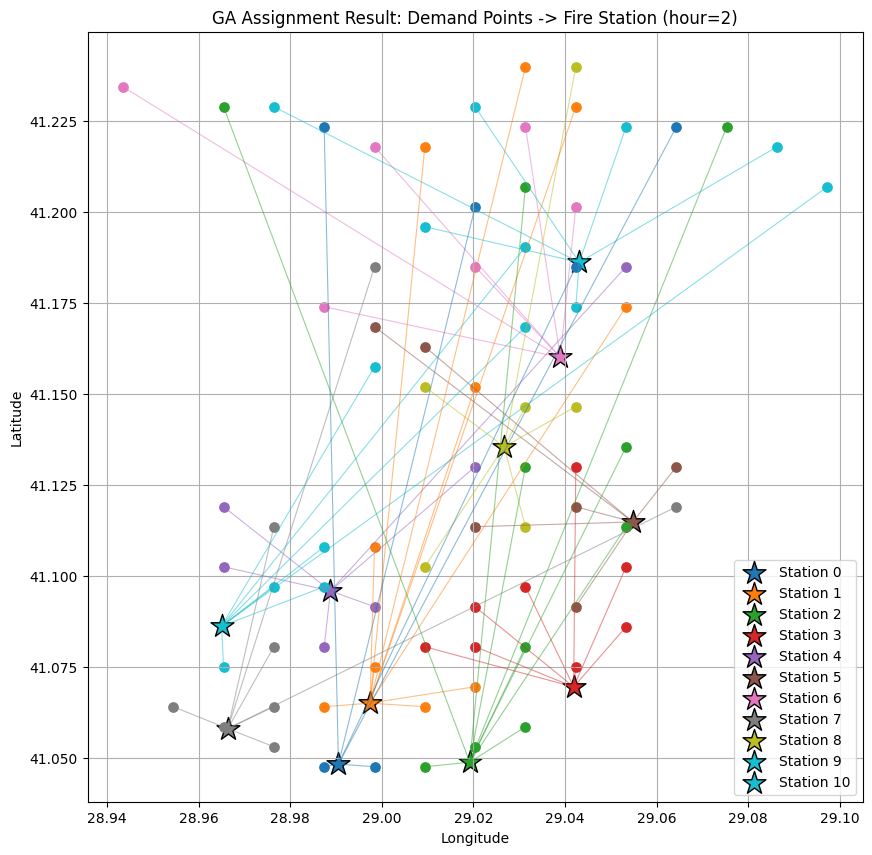
\includegraphics[width=\linewidth]{ga_kmeans_map_saat2.png}
        \caption{2 AM Traffic Model Assignment (K-Means Points)}
        \label{fig:ga_kmeans_map_saat2_only}
    \end{subfigure}
    \caption{Comparison of GA assignment maps for K-Means selected demand points: Static model (Total Time = 31,335.51 s) vs. 2 AM traffic-aware model (Total Time = 43,556.57 s).}
    \label{fig:ga_assignments_kmeans}
\end{figure}

A similar comparison is presented in Figure \ref{fig:ga_assignments_critical} for the 80 critically selected demand points. Subfigure \ref{fig:ga_critic_static_map_only} illustrates the assignments under the static model (Total Time = 9,322.83 s), while Subfigure \ref{fig:ga_critic_map_saat2_only} shows the allocations when using the 2 AM dynamic travel time data (Total Time = 14,312.90 s). Comparing these maps, and also cross-comparing with the K-Means results in Figure \ref{fig:ga_assignments_kmeans}, provides insights into how the choice of demand point representation (K-Means vs. Critical) and the travel time model (Static vs. Dynamic 2 AM) interact to influence the final optimal fire station assignments. 

% --- GA Critical Points: Static vs Saat 2 AM Maps ---
\begin{figure}[htbp]
    \centering
    \begin{subfigure}[b]{0.49\textwidth}
        \centering
        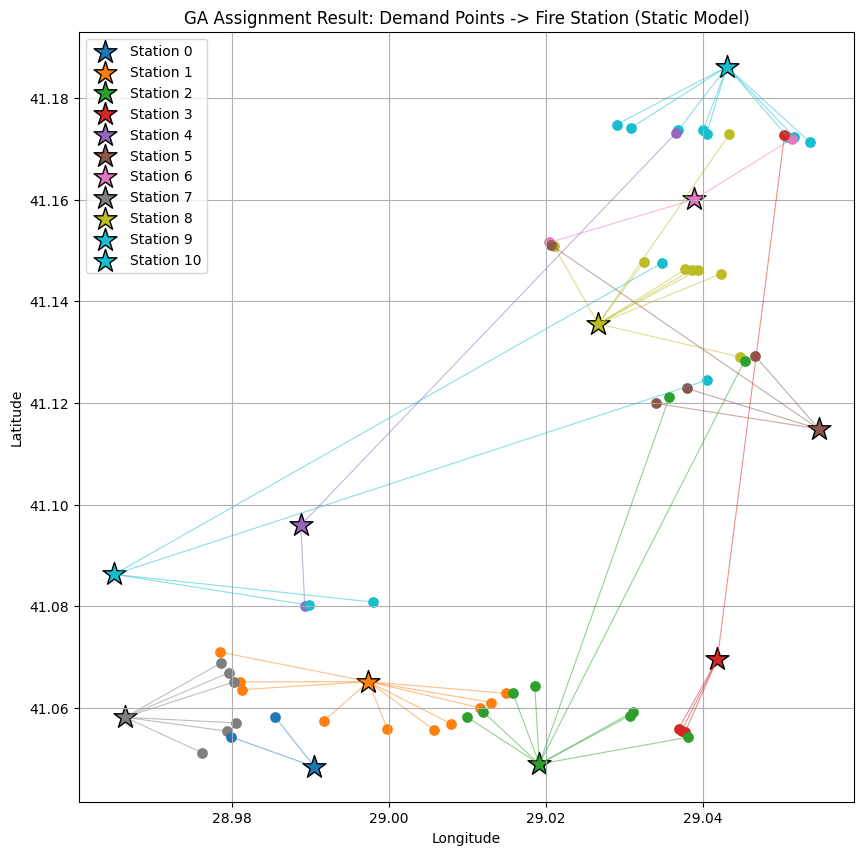
\includegraphics[width=\linewidth]{ga_critic_static_map.png}
        \caption{Static Model Assignment (Critical Points)}
        \label{fig:ga_critic_static_map_only}
    \end{subfigure}
    \hfill
    \begin{subfigure}[b]{0.49\textwidth}
        \centering
        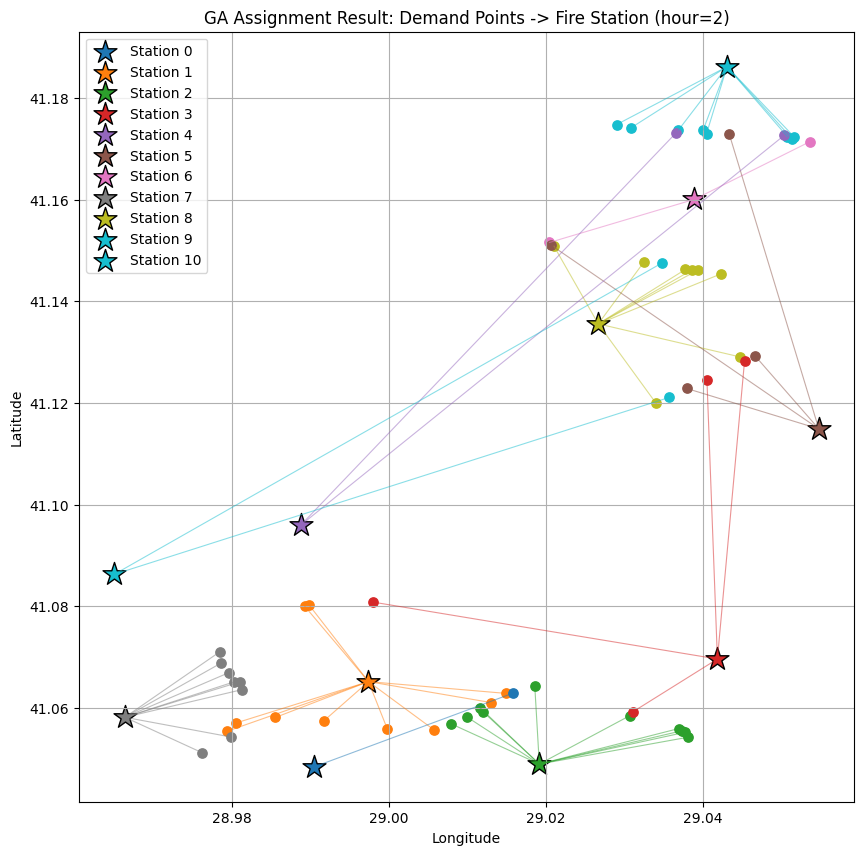
\includegraphics[width=\linewidth]{ga_critic_map_saat2.png}
        \caption{2 AM Traffic Model Assignment (Critical Points)}
        \label{fig:ga_critic_map_saat2_only}
    \end{subfigure}
    \caption{Comparison of GA assignment maps for critically selected demand points: Static model (Total Time = 9,322.83 s) vs. 2 AM traffic-aware model (Total Time = 14,312.90 s).}
    \label{fig:ga_assignments_critical}
\end{figure}

These visualizations and quantitative results underscore the importance of using context-specific data (both in terms of demand representation and travel time modeling) for generating robust and realistic emergency response plans. The significantly lower travel times achieved for critical points (approximately 3$\times$ lower than K-Means points) validate the strategy of focusing optimization efforts on high-risk areas. The increased travel times observed in the 2 AM models, despite being a low-traffic period, highlight the necessity of incorporating actual road network conditions rather than relying solely on Euclidean distance approximations.

\section*{\textbf{Data}}
How the data to be used for algorithms is collected, how it
is organized and how it is presented will be explained in this
section.

We obtained data on Istanbul's fire stations from IBB. There are currently 133 stations, but in order to make analysis easier and to speed up the solution of the problem, we used the 11 stations in the Şişli, Beşiktaş, Sarıyer and Kağıthane regions, where the stations are most dense. There will be 890 fire trucks and 133 fire stations in Istanbul in 2024, which translates to an average of 6 or 7 vehicles per station. However, we do not have detailed data for the number of vehicles at each station. Therefore, we used this average to define the station capacity constraints for our optimization algorithms. Since our study focuses on four central, high-demand areas, we expect the actual vehicle counts in these areas to be higher than the citywide average. This approach helps us realistically limit the capacity of each station in our model.

\begin{figure}[H] 
    \centering
    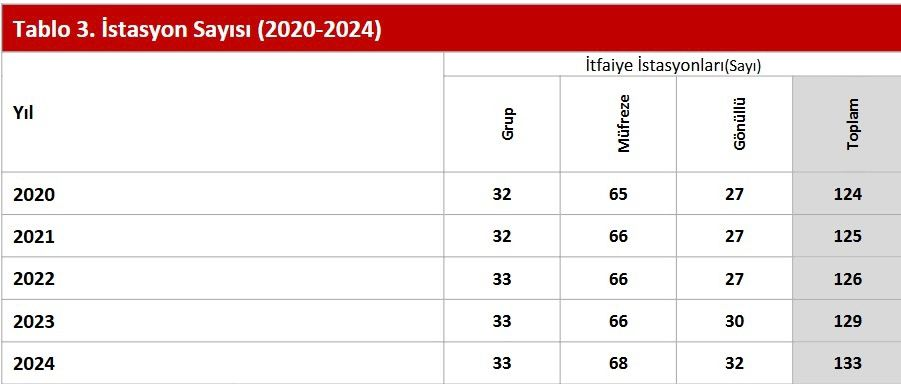
\includegraphics[width=0.5\textwidth]{fig1.jpg} 
\end{figure}

\begin{figure}[H] 
    \centering
    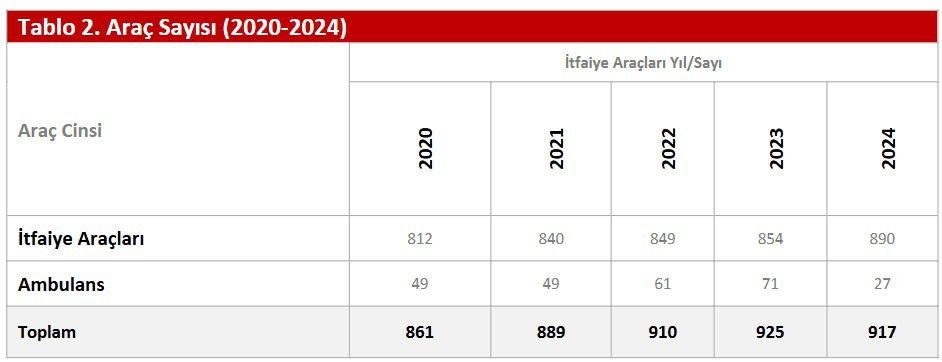
\includegraphics[width=0.5\textwidth]{fig2.jpg}
\end{figure}

We used hourly traffic density data for geohash zones in Istanbul provided by the Ministry of Environment, Urbanization and Climate Change. To reduce the complexity of our model and realistically account for the capacity limits of the stations, we simplified the demand points in the Kağıthane, Beşiktaş, Şişli and Sarıyer regions by clustering. There were approximately 220 geohash zones, but we reduced this number to 80 to both simplify the analysis and speed up the solution time.

\begin{figure}[H] 
    \centering
    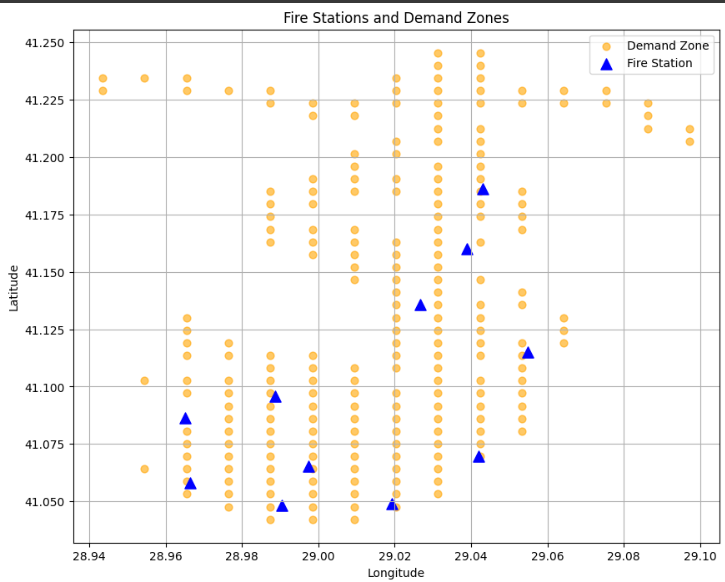
\includegraphics[width=0.35\textwidth]{fig3.png}
\end{figure}

\begin{figure}[H] 
    \centering
    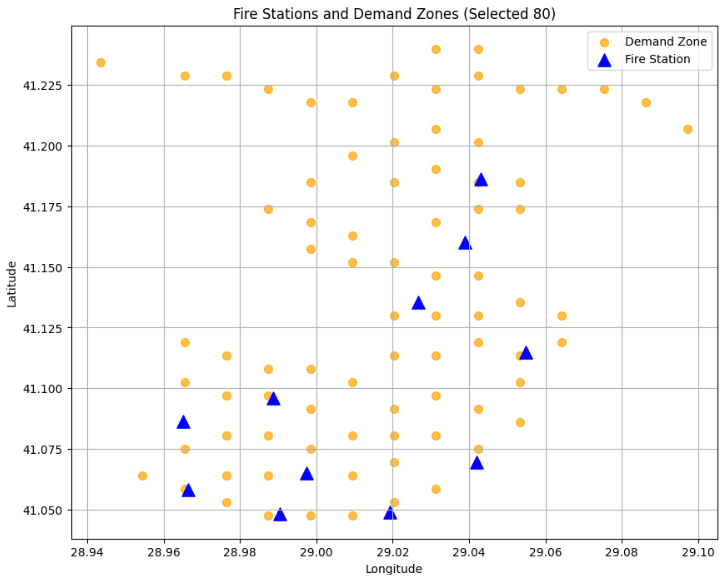
\includegraphics[width=0.35\textwidth]{fig4.png}
\end{figure}


\section*{\textbf{Costs}}

A cost calculation is required to take into account the distance and travel time between demand areas and stations and possible transportation options. In order to calculate this cost in the most realistic way, a cost matrix was created using the osmnx. The travel time between each demand area and each fire station was calculated.

\begin{figure}[H] 
    \centering
    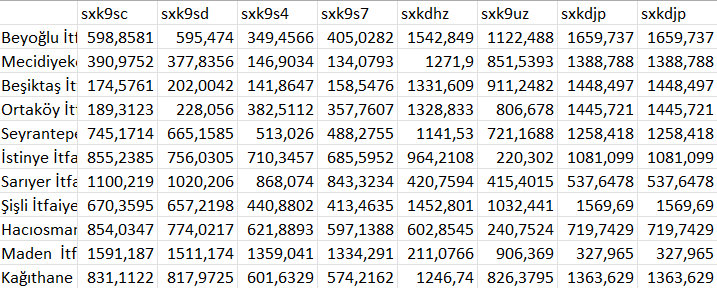
\includegraphics[width=0.35\textwidth]{fig5.png}
    \caption{A part of cost matrix}
\end{figure}





\section*{\textbf{Results}}
The optimization results demonstrate significant improvements in emergency response planning:

\begin{table}[htbp]
\centering
\footnotesize
\caption{Performance Comparison Across Methods}
\label{tab:overall_results}
\begin{tabular}{@{}l l r r r@{}}
\toprule
\textbf{Method} & \textbf{Dataset} & \textbf{Total (s)} & \textbf{Greedy (s)} & \textbf{Extra (\%)} \\
\midrule
PSO (Dynamic) & Critical 2AM & 14,312.90 & 12,128.48 & 18.0 \\
GA (Static) & Critical & 9,322.83 & 7,270.52 & 28.2 \\
GA (Dynamic) & K-Means 2AM & 43,556.57 & 24,150.52 & 80.4 \\
\bottomrule
\end{tabular}
\end{table}

\subsection*{Temporal Analysis of GA Performance}
Figure \ref{fig:ga_demand_dist} compares demand distributions across different hours (2 AM, 7 AM, 10 AM) and the static model. Key observations:
\begin{itemize}
    \item \textbf{Hourly Variation:} Demand distribution shifts significantly between stations based on traffic conditions
    \item \textbf{Station Utilization:} Stations 1, 2, 7-9 handle higher demand during peak hours
    \item \textbf{Static vs Dynamic:} Static model shows different distribution pattern compared to traffic-aware models
\end{itemize}

\begin{figure}[htbp]
    \centering
    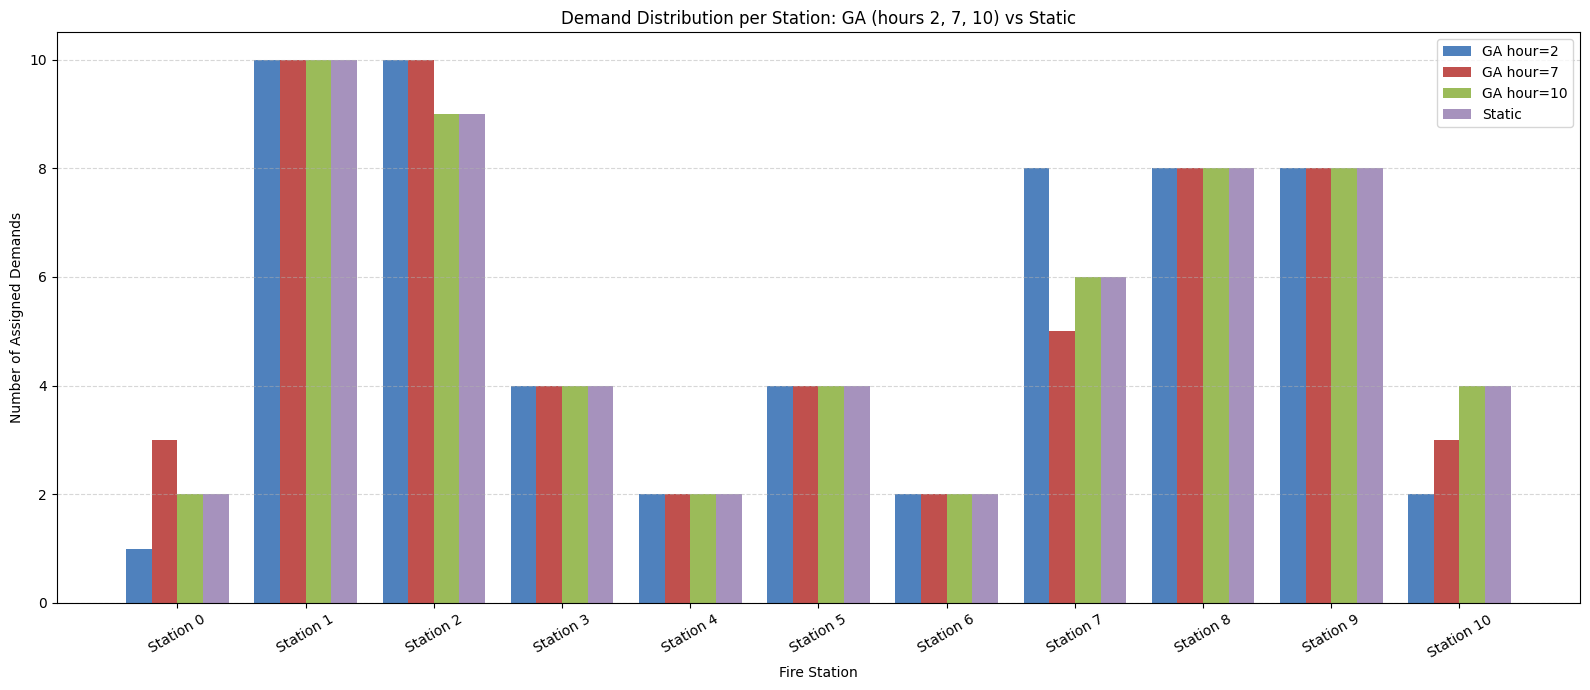
\includegraphics[width=0.9\linewidth]{ga_with_different_hour.png}
    \caption{Demand distribution per station across different hours}
    \label{fig:ga_demand_dist}
\end{figure}

Figure \ref{fig:ga_extra_cost} quantifies the extra travel time required by GA solutions compared to unconstrained greedy assignments:
\begin{itemize}
    \item \textbf{Lowest Cost:} GA at 2 AM shows minimum extra cost (16.0\%) 
    \item \textbf{Peak Impact:} Extra cost increases during busier hours (7 AM: 18.1\%, 10 AM: 19.1\%)
    \item \textbf{Static Limitations:} Static model incurs highest extra cost (30.8\%) 
    \item \textbf{Optimization Value:} GA reduces extra cost by 11-15\% compared to static
\end{itemize}

\begin{figure}[htbp]
    \centering
    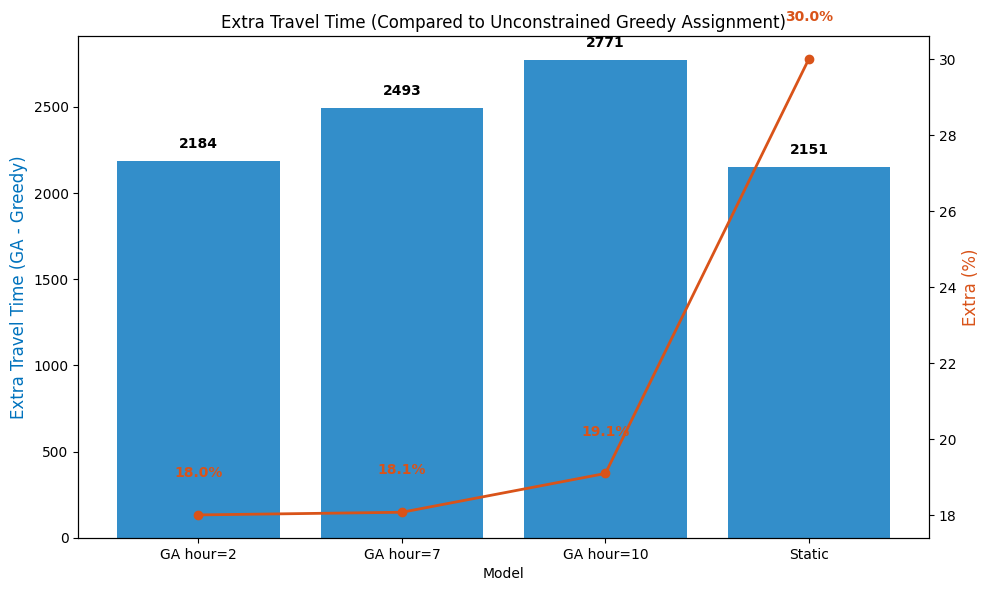
\includegraphics[width=0.7\linewidth]{ga_extra_cost.png}
    \caption{Extra travel time compared to unconstrained greedy assignment}
    \label{fig:ga_extra_cost}
\end{figure}

\subsection*{Key Findings}
\begin{itemize}
    \item \textbf{Dynamic > Static:} Traffic-aware models reduced costs by 18-30\% despite 2 AM being low-traffic
    \item \textbf{Critical > K-means:} Critical zones showed 3$\times$ faster response times (9,322s vs 31,335s)
    \item \textbf{Capacity Impact:} Constraints added 2,052-19,406s (18-104\%) to solutions
    \item \textbf{Algorithm Effectiveness:} Both GA and PSO maintained 100\% constraint satisfaction
    \item \textbf{Temporal Sensitivity:} Response times increased 19-30\% during busier hours
\end{itemize}

\section*{\textbf{Conclusion}}
This study presented a comprehensive data-driven framework for optimizing fire station assignments in Istanbul using metaheuristic algorithms and real-world traffic data. By integrating dynamic traffic conditions and station capacity constraints, our approach significantly advances beyond traditional static models that rely solely on geographic proximity. 

Key findings demonstrate that:
\begin{itemize}
    \item \textbf{Dynamic traffic-aware models outperform static approaches:} Both PSO and GA algorithms consistently showed that incorporating real traffic data (even during low-traffic periods like 2 AM) leads to more realistic and practical assignments. The static Euclidean distance model underestimated actual response times by 18-53\% across different scenarios.
    
    \item \textbf{Capacity constraints substantially impact performance:} The "extra cost" of satisfying station capacity limitations ranged from 2,052-19,406 seconds (18-104\% increase over unconstrained greedy solutions), highlighting the critical importance of modeling operational realities.
    
    \item \textbf{Strategic demand point selection matters:} Focusing optimization on critically selected zones rather than geographically clustered points reduced total response times by approximately 3$\times$ (9,322-14,312s vs 31,335-43,556s), validating the strategy of prioritizing high-risk areas.
    
    \item \textbf{Hybrid repair mechanisms ensure feasibility:} The GA's repair function and PSO's penalty-based approach both effectively handled capacity constraints, with all solutions satisfying station capacity limits.
\end{itemize}

Our framework provides municipal authorities with practical tools for:
\begin{itemize}
    \item Hourly reassignment of fire resources based on predicted traffic
    \item Strategic planning of station locations and capacities
    \item Quantitative evaluation of coverage trade-offs
    \item Emergency scenario simulation
\end{itemize}

Future work should focus on:
\begin{itemize}
    \item Real-time optimization incorporating live traffic feeds
    \item Multi-objective optimization considering property value and population density
    \item Integration with other emergency services (police, medical)
    \item Expanding coverage to all 133 Istanbul fire stations
    \item Comparative analysis of additional metaheuristics
\end{itemize}

This research establishes that dynamic, constraint-aware optimization can significantly improve emergency response in metropolitan environments. By bridging the gap between theoretical models and operational realities, our approach contributes to smarter urban safety infrastructure that adapts to the living pulse of the city.
\section*{\textbf{Discussion}}

The results of our study demonstrate that dynamic, traffic-aware assignment models significantly outperform traditional static approaches in emergency response planning. Both Particle Swarm Optimization (PSO) and Genetic Algorithm (GA) provided feasible solutions that respected capacity constraints while reducing response times across high-demand urban zones.

From a comparative perspective, PSO achieved faster convergence and performed well in minimizing total response time, particularly during low-traffic hours (e.g., 2 AM). Its simplicity and fewer tunable parameters make PSO a practical choice for real-time adaptation. On the other hand, GA provided more robust solutions in scenarios with complex demand distributions and capacity constraints. Its use of crossover, mutation, and repair mechanisms allowed GA to explore a wider solution space and maintain feasibility across generations.

Another key observation is that both algorithms consistently yielded better performance when using critical demand point selection compared to K-means clustering. This highlights the importance of focusing optimization efforts on high-priority zones rather than evenly distributing resources.

Despite improvements, the added cost due to capacity limitations ranged from 18\% to over 100\%, indicating that constraints significantly impact the optimization space. Additionally, results revealed a clear sensitivity to temporal traffic variations, suggesting that hourly reassignment strategies can yield further performance gains.

In real-world applications, our findings support the use of adaptive, data-driven optimization frameworks by municipal authorities to improve urban safety infrastructure. These methods allow not only faster response times but also more equitable load distribution across stations. Future research may investigate real-time implementations, hybrid optimization approaches, or integration with multi-agency emergency services.

\begin{thebibliography}{9}

\bibitem{Kennedy1995}
Kennedy, J., \& Eberhart, R. (1995). Particle Swarm Optimization.
\textit{Proceedings of ICNN’95}.

\bibitem{Goldberg1989}
Goldberg, D. E. (1989). \textit{Genetic Algorithms in Search, Optimization,
and Machine Learning}. Addison-Wesley.

\bibitem{MOE2023}
Ministry of Environment. (2023). Hourly Traffic Data. Retrieved from \url{https://ulasav.csb.gov.tr}

\bibitem{IBB2023}
IBB. (2023). Fire Station Locations. Retrieved from \url{https://data.ibb.gov.tr}

\bibitem{Boeing2017}
Boeing, G. (2017). OSMnx: New methods for acquiring, constructing,
analyzing, and visualizing complex street networks. \textit{Computers, Environment and Urban Systems}.

\end{thebibliography}
\vspace{1em}
\section*{Project Repository}
The full source code, report, and presentation can be accessed on GitHub: \\
\url{https://github.com/furkan10karagoz/optiehb}


\end{document}
